% ======================================================================
% MNRAS paper draft (full rewrite, 2026-04-24)
%
% Central scientific claim:
%   Direct sampling under a flat-in-redshift distance prior produces a
%   materially different GW170817 H_0 posterior than post-hoc reweighting
%   of the baseline volumetric-distance posterior. The difference is
%   driven by the poor baseline coverage of the low-d_L region that the
%   flat-in-redshift prior up-weights. GPU-accelerated nested sampling
%   makes such direct prior-sensitivity checks practical.
%
% Every numerical claim in the Results/Performance sections must be
% traceable to a repository file. Drafting notes of the form
%   [Source: Results/.../file.csv]
% are retained for the co-author review pass and are intended to be
% removed before journal submission.
% ======================================================================

\documentclass[fleqn,usenatbib]{mnras}

\usepackage[T1]{fontenc}
\usepackage{newtxtext,newtxmath}
\usepackage{graphicx}
\usepackage{amsmath}
\usepackage{booktabs}
\usepackage{url}
\usepackage{xspace}

\graphicspath{{../Results/gwtc1_phasemarg/plots/}{Results/gwtc1_phasemarg/plots/}}

\newcommand{\kmsmpc}{\ensuremath{\,\rm km\,s^{-1}\,Mpc^{-1}}\xspace}
\newcommand{\kms}{\ensuremath{\,\rm km\,s^{-1}}\xspace}
\newcommand{\hzero}{\ensuremath{H_{0}}\xspace}
\newcommand{\dL}{\ensuremath{d_{L}}\xspace}
\newcommand{\sigmavp}{\ensuremath{\sigma_{v_p}}\xspace}
\newcommand{\IMR}{IMRPhenomD\_NRTidalv2\xspace}
\newcommand{\TF}{TaylorF2\xspace}
\newcommand{\bjns}{\textsc{blackjax-ns}\xspace}
\newcommand{\bilby}{\textsc{bilby}\xspace}
\newcommand{\pbilby}{\textsc{parallel\_bilby}\xspace}
\newcommand{\jax}{\textsc{jax}\xspace}
\newcommand{\ripple}{\textsc{ripple}\xspace}

\title[Rapid GW170817 \hzero inference]{Rapid Hubble constant inference from GW170817 using GPU-accelerated nested sampling}

\author[M. Yang et al.]{
Ming Yang,$^{1}$\thanks{E-mail: TODO}
Will Handley,$^{2,3}$
and \mbox{TODO co-authors}
\\
$^{1}$St John's College, University of Cambridge, Cambridge CB2 1TP, UK\\
$^{2}$Institute of Astronomy, University of Cambridge, Madingley Road, Cambridge CB3 0HA, UK\\
$^{3}$Kavli Institute for Cosmology, University of Cambridge, Madingley Road, Cambridge CB3 0HA, UK
}

\date{Accepted XXX. Received YYY; in original form ZZZ}
\pubyear{2026}

\begin{document}
\label{firstpage}
\pagerange{\pageref{firstpage}--\pageref{lastpage}}
\maketitle

% ======================================================================
\begin{abstract}
The binary neutron-star merger GW170817 remains the only confirmed bright gravitational-wave standard siren, and the reference event for direct measurements of the Hubble constant, \hzero, from a compact-binary coalescence. The scientific usefulness of a single bright-siren \hzero posterior depends sensitively on the assumed distance, redshift, and host peculiar-velocity priors, and a complete robustness study requires repeated full parameter estimation under each choice. We revisit GW170817 with a GPU-native nested-sampling pipeline that combines a heterodyned likelihood with differentiable \jax waveforms, and use it to carry out a direct prior-sensitivity study. Our primary \IMR run with 5000 live points recovers a broad \hzero posterior with maximum-posterior value $71.5\kmsmpc$ and weighted 68 per cent quantile interval $[68.2,103.5]\kmsmpc$, consistent with the original GW170817 bright-siren measurement. Replacing the volumetric distance prior with a flat-in-redshift prior by direct sampling shifts the weighted median from $79.1$ to $93.6\kmsmpc$ and raises the tail probability $P(\hzero>120\kmsmpc)$ from $0.076$ to $0.281$. Post-hoc reweighting of the baseline posterior to the same target prior yields $0.195$, partially capturing the shift but understating the high-\hzero tail. The mechanism is visible in the luminosity-distance marginal, where the direct run samples the low-\dL region that the baseline volumetric prior under-populates. Waveform variation between \IMR and \TF, and a change in the host peculiar-velocity uncertainty from $150$ to $250\kms$, both produce smaller shifts than the distance-prior effect. The full 5000-live-point analysis completes in 14\,min 45\,s on a single NVIDIA A100 GPU, and the six-run prior suite in 57\,min, making direct prior and waveform robustness checks practical for bright-siren cosmology.
\end{abstract}

\begin{keywords}
gravitational waves -- methods: data analysis -- cosmological parameters -- stars: neutron -- software: data analysis
\end{keywords}

% ======================================================================
\section{Introduction}
\label{sec:introduction}

The present-day expansion rate of the Universe, quantified by the Hubble constant \hzero, is the subject of one of the most persistent tensions in contemporary cosmology. Measurements anchored in the early Universe, derived from cosmic-microwave-background observations assuming flat $\Lambda$CDM, favour a relatively low value \citep{Planck2016}, while late-Universe distance-ladder measurements based on Cepheids and Type Ia supernovae find a significantly higher value \citep{Riess2016,Riess2022}. The statistical and systematic discrepancy between these two families of measurement is now established at several $\sigma$, and its resolution, whether through unrecognised systematics or new cosmological physics, motivates independent probes of the expansion rate.

Gravitational-wave standard sirens are such a probe. The waveform amplitude of a compact-binary merger fixes the luminosity distance directly, without reference to an astrophysical distance ladder \citep{Schutz1986}. When the merger is accompanied by an electromagnetic counterpart that identifies a host galaxy, the host redshift can be combined with the gravitational-wave distance to infer \hzero from a single event. The binary neutron-star merger GW170817 \citep{Abbott2017GW170817Discovery} is the canonical bright siren and the only confirmed example to date. Its association with the kilonova AT2017gfo in NGC 4993 provided the host-galaxy redshift needed to yield the first gravitational-wave measurement of \hzero \citep{Abbott2017H0}.

For a bright siren, the \hzero uncertainty is dominated by the luminosity-distance--inclination degeneracy: a face-on binary at larger \dL can produce the same observed strain as a more inclined binary at smaller \dL, with the two solutions mapping to different values of $\hzero = v_{\rm r}/\dL$ for a fixed host recessional velocity $v_{\rm r}$. The resulting posterior is broad, skewed, and only weakly informative on \hzero from one event. In such a regime, the measurement is more sensitive to prior choices than the statistical uncertainty alone would suggest, because the prior shapes the tails of the posterior rather than just its peak. The original GW170817 analysis assumed a volumetric distance prior $\pi(\dL)\propto\dL^{2}$ and reported that switching to a flat-in-redshift prior, implemented by reweighting posterior samples, produced only a minor change in the inferred \hzero posterior \citep{Abbott2017H0}.

Reweighting is attractive because it avoids rerunning expensive Bayesian inference. For a source-parameter posterior $p(\theta\mid d,\pi_{0})$ obtained under baseline prior $\pi_{0}$, the target posterior under an alternative prior $\pi_{1}$ can be estimated by assigning each posterior sample a weight proportional to $\pi_{1}(\theta)/\pi_{0}(\theta)$. This procedure is statistically consistent provided that the baseline samples cover the support of the target posterior; if $\pi_{1}/\pi_{0}$ is large in regions that the baseline run has sampled sparsely, the reweighted estimator has high variance and systematically low tail mass \citep[see e.g.][for a general discussion of reweighting in the nested-sampling context]{Speagle2020Dynesty}. For GW170817, the baseline volumetric prior $\pi_{0}(\dL)\propto\dL^{2}$ places little mass at the low \dL values corresponding to the top of the \hzero prior range; a flat-in-redshift target prior up-weights exactly this region, and the validity of reweighting is not obvious a priori.

Testing reweighting against a direct posterior obtained by sampling under the target prior requires repeated full gravitational-wave parameter estimation. In CPU-based frameworks such as \bilby \citep{Ashton2019Bilby} and its parallelised counterpart \pbilby, a single 128\,s binary-neutron-star analysis with phase-marginalised frequency-domain likelihood costs hundreds of CPU core-hours to thousands of core-hours, depending on waveform, live-point count, and prior bounds. Systematic exploration of distance, velocity, and waveform assumptions therefore becomes prohibitive. This computational cost is not only a practical nuisance: it directly limits the robustness studies that can be performed for a bright-siren cosmological result.

Several recent developments make this constraint less severe. Relative binning, also known as the heterodyned likelihood \citep{Cornish2013,Zackay2018RelativeBinning}, reduces the effective frequency grid for a long inspiral to a small number of bins with negligible loss of accuracy. Differentiable waveform libraries in \jax \citep{Bradbury2018JAX}, including \ripple \citep{Edwards2023Ripple}, enable end-to-end GPU evaluation of the likelihood. GPU-native nested-sampling kernels \citep{BlackJAX,Yallup2025BlackJAXNS,Prathaban2025GPUSpeed} retain the evidence estimates that nested sampling provides for free while allowing large live-point counts and repeated full reruns. Related efforts have demonstrated accelerated binary-neutron-star inference with related tools \citep{Krishna2023RelativeBinningBilby,Wong2023Jim,Wouters2024JimBNS}, and have underlined the practical importance of compute-efficient parameter estimation for the third-generation detector era \citep{HuVeitch2025}.

In this paper we use a GPU-native nested-sampling pipeline, built on \bjns \citep{Yallup2025BlackJAXNS,Prathaban2025GPUSpeed} and a \jax implementation of the heterodyned likelihood, to revisit the GW170817 bright-siren \hzero inference. Our focus is not a new single-event measurement of \hzero, but a controlled assessment of how that measurement depends on its priors. We first validate the pipeline against GW150914 and against reference GW170817 posteriors. We then report the baseline \hzero posterior, compare it with a direct flat-in-redshift posterior and with the reweighted flat-in-redshift posterior obtained from the baseline samples, and quantify the prior sensitivity and the waveform cross-check. We finish by reporting runtime and live-point scaling on a single A100 GPU. Performance is presented to motivate that the prior-sensitivity study is now tractable, not as a central claim of the paper.

Section~\ref{sec:method} describes the inference setup. Section~\ref{sec:validation} reports validation. Section~\ref{sec:results} contains the \hzero inference and the prior-sensitivity analysis. Section~\ref{sec:performance} reports runtime and scaling. Section~\ref{sec:discussion} discusses implications and limitations. Section~\ref{sec:conclusions} concludes.

% ======================================================================
\section{Method}
\label{sec:method}

\subsection{Nested sampling}

For data $d$ and source parameters $\theta$ under model $\mathcal{M}$, we target the posterior
\begin{equation}
p(\theta\mid d,\mathcal{M}) = \frac{\mathcal{L}(d\mid\theta,\mathcal{M})\,\pi(\theta\mid\mathcal{M})}{Z(d\mid\mathcal{M})},
\label{eq:bayes}
\end{equation}
where $\mathcal{L}$ is the gravitational-wave likelihood, $\pi$ the prior, and $Z$ the Bayesian evidence. We estimate $Z$ and draw posterior samples by nested sampling \citep{Skilling2006Nested}, using the GPU-native slice sampler implemented in \bjns \citep{Yallup2025BlackJAXNS,Prathaban2025GPUSpeed}. The sampler evolves a population of live points through batched slice updates; this vectorisation is the key ingredient that keeps the GPU saturated when the per-evaluation likelihood cost is small.

All heterodyned GW170817 runs in this paper use $n_{\rm live}=5000$, $n_{\rm delete}=2500$ points removed per iteration ($\tfrac12\,n_{\rm live}$), and $5\,n_{\rm dim}$ MCMC steps per slice; runs terminate when the fractional evidence increment is below $10^{-3}$ [Source: \texttt{paper\_knowledge\_base/a100\_run\_data.md}, \texttt{paper\_knowledge\_base/codebase\_reference.md}]. Scaling experiments vary $n_{\rm live}$ while holding all other settings fixed.

\subsection{Heterodyned likelihood}

The GW170817 signal is long enough that the full frequency-domain likelihood uses $259\,201$ bins over $20$--$2048\,\rm Hz$ with $\Delta f=1/128\,\rm Hz$ for the $128\,\rm s$ strain segment [Source: \texttt{paper\_knowledge\_base/codebase\_reference.md}]. Evaluating the likelihood on this grid for every live-point update is prohibitively expensive when millions of evaluations are required. We therefore use a heterodyned (relative-binning) likelihood \citep{Cornish2013,Zackay2018RelativeBinning}, in which the ratio between a candidate waveform and a reference waveform is approximated by a piecewise-linear function over a small set of coarse frequency bins. We use $501$ nominal heterodyne bins, of which the effective count is $442$ for \TF and $501$ for \IMR after waveform-specific frequency-support masks are applied [Source: \texttt{paper\_knowledge\_base/a100\_run\_data.md}]; for GW150914, $383$ bins are used [Source: same]. The reference waveform uses the GWTC-1 median posterior parameters for GW170817.

We compare heterodyned and unheterodyned posteriors directly in Section~\ref{sec:validation} to verify that the approximation does not bias the source-parameter posterior at the level needed for \hzero inference. All reported heterodyned runs also marginalise analytically over the coalescence phase, so the sampled parameter space is fourteen-dimensional for GW170817 (intrinsic masses, spin $z$-components, tidal deformabilities, inclination, luminosity distance, coalescence time, polarisation angle, sky position, and the cosmological parameters $\hzero$ and $v_p$), and ten-dimensional for GW150914.

\subsection{Joint Hubble-constant likelihood}

We sample the Hubble constant jointly with the gravitational-wave source parameters rather than post-processing the \dL marginal. The GW170817 host galaxy NGC~4993 provides a CMB-frame recessional velocity $v_{\rm r}$ and a Hubble-flow peculiar-velocity estimate $\langle v_{p}\rangle$; both are used as Gaussian likelihoods on the model prediction. The combined log-likelihood is
\begin{equation}
\ln\mathcal{L}_{\rm tot}(\theta,\hzero,v_{p}) = \ln\mathcal{L}_{\rm GW}(d\mid\theta) + \ln p(v_{\rm r}\mid\hzero\,\dL+v_{p}) + \ln p(\langle v_{p}\rangle\mid v_{p}),
\label{eq:h0likelihood}
\end{equation}
where $\dL$ is a function of $\theta$ only, and $\hzero$ and $v_{p}$ enter through the velocity terms alone. This is the standard GW170817 bright-siren setup, following \citet{Abbott2017H0}.

\subsection{Priors and prior variants}

The baseline prior configuration follows the GW170817 bright-siren analysis: $\pi(\dL)\propto\dL^{2}$ over $[10,75]\,\rm Mpc$, $\pi(\hzero)\propto\hzero^{-1}$ over $[45,250]\kmsmpc$, and $\pi(v_{p})$ uniform over $[-1000,1000]\kms$ with a Gaussian centred on $\langle v_{p}\rangle$ at $\sigmavp=150\kms$ in the peculiar-velocity likelihood term. Source-parameter priors are the constrained ``host-localised'' set implemented in \texttt{GW170817\_heterodyned\_1.py}: narrow ranges on chirp mass, mass ratio, and aligned-spin $z$-components around the GWTC-1 reference values, a uniform tidal prior, and a narrow sky-location prior centred on NGC~4993 [Source: \texttt{paper\_knowledge\_base/codebase\_reference.md}].

We consider three prior variants in addition to the baseline:
\begin{enumerate}
    \item \emph{Direct flat-in-redshift}: $\pi(z)$ uniform within the corresponding distance range, converted to a \dL prior via a flat $\Lambda$CDM cosmology and sampled directly (\texttt{GW170817\_heterodyned\_2.py}).
    \item \emph{Reweighted flat-in-redshift}: the baseline posterior samples reweighted by the analytic ratio of the flat-in-redshift to volumetric \dL priors (\texttt{Plots/reweight\_dL\_to\_flat\_z.py}).
    \item \emph{Enlarged peculiar-velocity uncertainty}: identical to the baseline except $\sigmavp=250\kms$ (\texttt{GW170817\_heterodyned\_3.py}).
\end{enumerate}
The direct and reweighted flat-in-redshift posteriors use the same target prior, and differ only in whether the prior is imposed during sampling or applied post-hoc.

\subsection{Waveforms}

Our primary gravitational-wave model is \IMR, an aligned-spin tidal waveform available in the differentiable \ripple library \citep{Edwards2023Ripple}. We use \TF as a waveform cross-check; our implementation is a point-particle post-Newtonian inspiral-only model, without tidal corrections, and its agreement with the primary analysis is a test for waveform systematics in the distance--inclination plane rather than a like-for-like tidal comparison. The original GW170817 bright-siren analysis used IMRPhenomPv2\_NRTidal, which includes precession. The aligned-spin approximation is expected to be adequate for this event because NGC~4993 pins the sky location and the informative direction on the distance posterior is the inclination at fixed polarisation, but we return to this limitation in Section~\ref{sec:discussion}.

% ======================================================================
\section{Validation}
\label{sec:validation}

\subsection{GW150914}

We validate the pipeline on the binary-black-hole event GW150914 \citep{Abbott2016GW150914}, which has a short signal and established public posteriors. We analyse the GWOSC strain data with IMRPhenomD and GWTC-2.1 PSDs, using the same heterodyned sampler as for GW170817 with 5000 live points and phase marginalisation. Table~\ref{tab:gw150914} summarises the recovered parameters. Chirp mass and luminosity distance are both recovered at values consistent with the GWTC reference, with broad inclination and spin posteriors as expected at the signal-to-noise ratio of GW150914. Figure~\ref{fig:gw150914} shows the corresponding corner plot against public GWTC-2.1 samples. The sampler returns $\ln Z = 260.95\pm0.08$ with $1.33\times10^{5}$ dead points [Source: \texttt{Results/gwtc1\_phasemarg/evidence\_table.csv}].

\begin{table}
  \centering
  \caption{Heterodyned GW150914 validation with IMRPhenomD and 5000 live points. MAP, weighted median, and weighted 68 per cent quantile intervals are shown.}
  \label{tab:gw150914}
  \begin{tabular}{lccc}
    \toprule
    Parameter & MAP & Median & 68\% interval \\
    \midrule
    $\mathcal{M}_{c}/M_{\odot}$ & 29.88 & 30.04 & $[29.10,31.12]$ \\
    $q$ & 0.93 & 0.83 & $[0.69,0.95]$ \\
    $\dL/\rm Mpc$ & 409.7 & 404.6 & $[289.6,509.6]$ \\
    $\iota/\rm rad$ & 2.62 & 2.49 & $[2.08,2.81]$ \\
    \bottomrule
  \end{tabular}
  \\ \footnotesize[Source: \texttt{Results/gwtc1\_phasemarg/summary\_stats.csv}.]
\end{table}

\begin{figure}
  \centering
  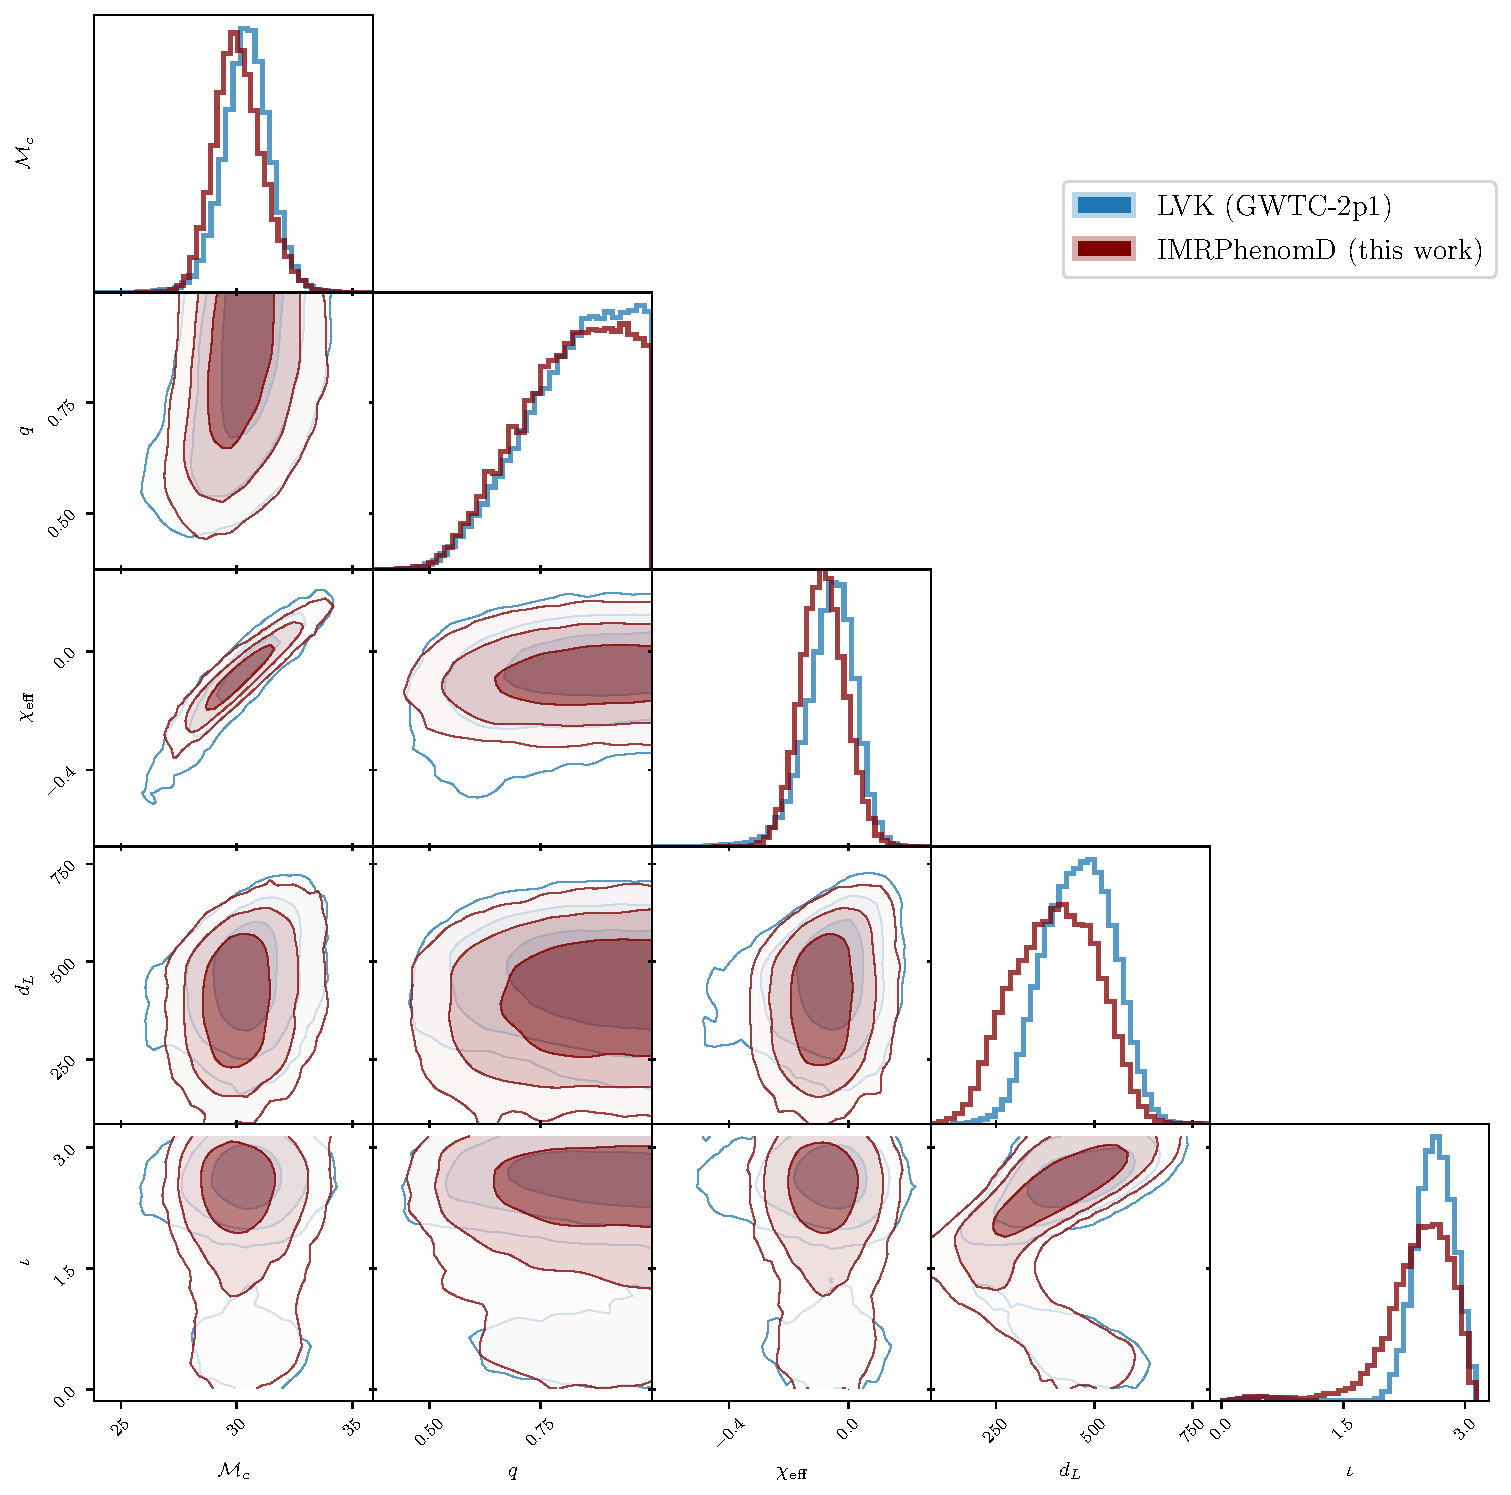
\includegraphics[width=\columnwidth]{corner_GW150914.pdf}
  \caption{GW150914 validation: pipeline posterior overlaid on public GWTC-2.1 samples for the principal source parameters. Priors and PSDs differ between the two analyses; the figure is intended to show qualitative agreement in the mass and distance structure, not a like-for-like reproduction. Produced by \texttt{Plots/plot\_GW150914.py} from \texttt{Results/gwtc1\_phasemarg/GW15\_PhaseMarg\_Heterodyned\_IMRPhenomD\_local\_psd-gwtc2p1\_ref-gwtc1.csv}.}
  \label{fig:gw150914}
\end{figure}

\subsection{Heterodyned versus unheterodyned consistency on GW170817}

We next check that the heterodyned approximation does not bias the GW170817 source-parameter posterior. We run the same sampler on the full $259\,201$-bin frequency-domain likelihood with host-localised priors for both \IMR and \TF, at a reduced 1500 live points to keep the runtime tractable [Source: \texttt{paper\_knowledge\_base/codebase\_reference.md}]. Table~\ref{tab:hetero-vs-unhet} compares key marginals. The heterodyned baseline and the unheterodyned run agree on the chirp mass to within the sampler width, and on the weighted median distance to better than one megaparsec. The heterodyned weighted median \hzero is $79.1\kmsmpc$, compared with $77.8\kmsmpc$ for the unheterodyned run, a shift that is much smaller than the statistical width of the \hzero posterior. Figure~\ref{fig:hetero} shows the corresponding corner comparison. We conclude that the heterodyned approximation is adequate for \hzero inference at this event's signal-to-noise ratio; the order-of-magnitude runtime reduction it provides is quantified in Section~\ref{sec:performance}.

\begin{table}
  \centering
  \caption{Heterodyned versus unheterodyned GW170817 posteriors with \IMR, host-localised priors. Weighted medians and 68 per cent quantile intervals are shown.}
  \label{tab:hetero-vs-unhet}
  \begin{tabular}{lcc}
    \toprule
    Parameter & Heterodyned & Unheterodyned \\
    \midrule
    $\hzero$ median $/\kmsmpc$ & 79.1 & 77.8 \\
    $\hzero$ 68\% $/\kmsmpc$ & $[68.2,103.5]$ & $[67.3,100.9]$ \\
    $\dL$ median /Mpc & 38.1 & 38.9 \\
    $\dL$ 68\% /Mpc & $[29.2,43.7]$ & $[30.0,44.3]$ \\
    $\iota$ median /rad & 2.55 & 2.55 \\
    \bottomrule
  \end{tabular}
  \\ \footnotesize[Source: \texttt{Results/gwtc1\_phasemarg/summary\_stats.csv}; heterodyned run is the \IMR baseline and unheterodyned run is \texttt{PhaseMarg\_Unheterodyned\_IMRPhenomD\_NRTidalv2\_local\_psd-gwtc1.csv}.]
\end{table}

\begin{figure}
  \centering
  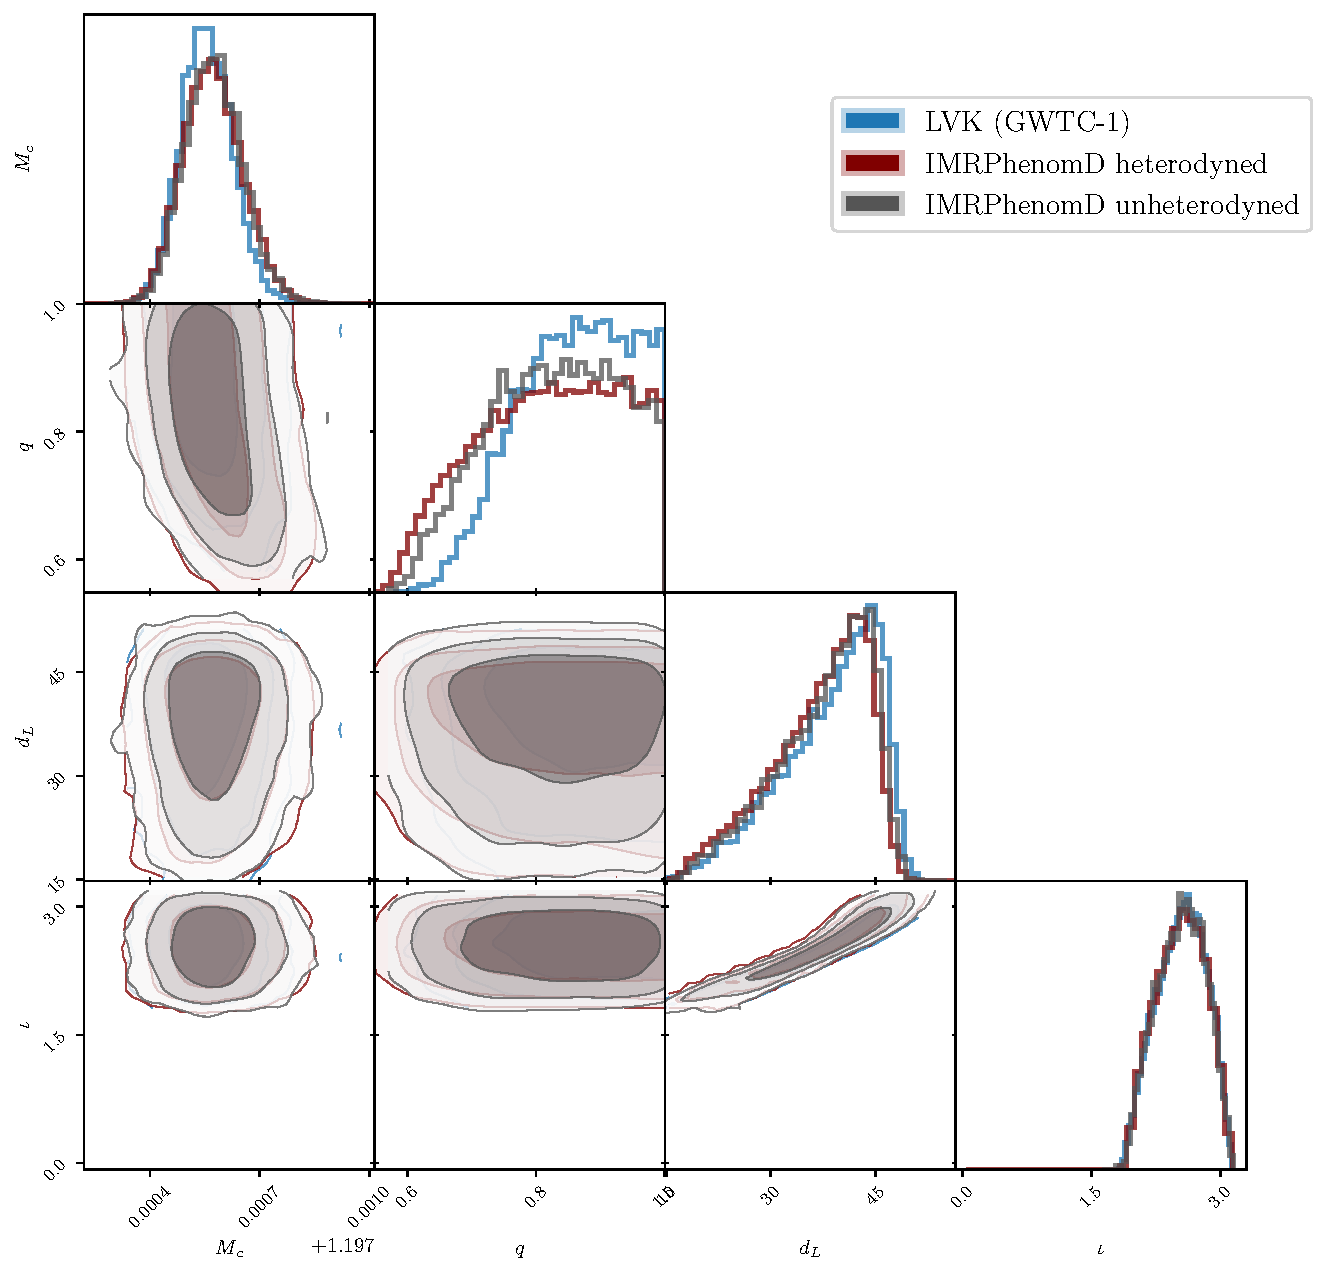
\includegraphics[width=\columnwidth]{corner_IMRPhenomD_hetero_vs_unhetero.pdf}
  \caption{GW170817 posterior comparison between the heterodyned baseline (501 bins, 5000 live points) and an unheterodyned reference run (full $259\,201$ bins, 1500 live points) under identical host-localised priors. GWTC-1 reference samples are overlaid for context. Produced by \texttt{Plots/plot\_corner\_IMRPhenomD\_hetero\_vs\_unhetero.py}.}
  \label{fig:hetero}
\end{figure}

\subsection{Cross-waveform consistency}

Figure~\ref{fig:combined} compares the \IMR and \TF heterodyned posteriors with the GWTC-1 reference samples. The JAX-based analyses recover the same distance--inclination structure as the LVK reference, with the known small offsets expected from the different waveform families and prior bounds. Jensen--Shannon divergences between the IMR and TF2 baseline posteriors are $0.0047\,\rm nats$ for \hzero and $0.0057\,\rm nats$ for \dL [Source: \texttt{Results/gwtc1\_phasemarg/waveform\_systematics.csv}], which is an order of magnitude smaller than the JSD values observed across prior variants in Section~\ref{sec:results}. Waveform systematics between our aligned-spin choices are therefore not the dominant source of uncertainty in the present analysis.

\begin{figure*}
  \centering
  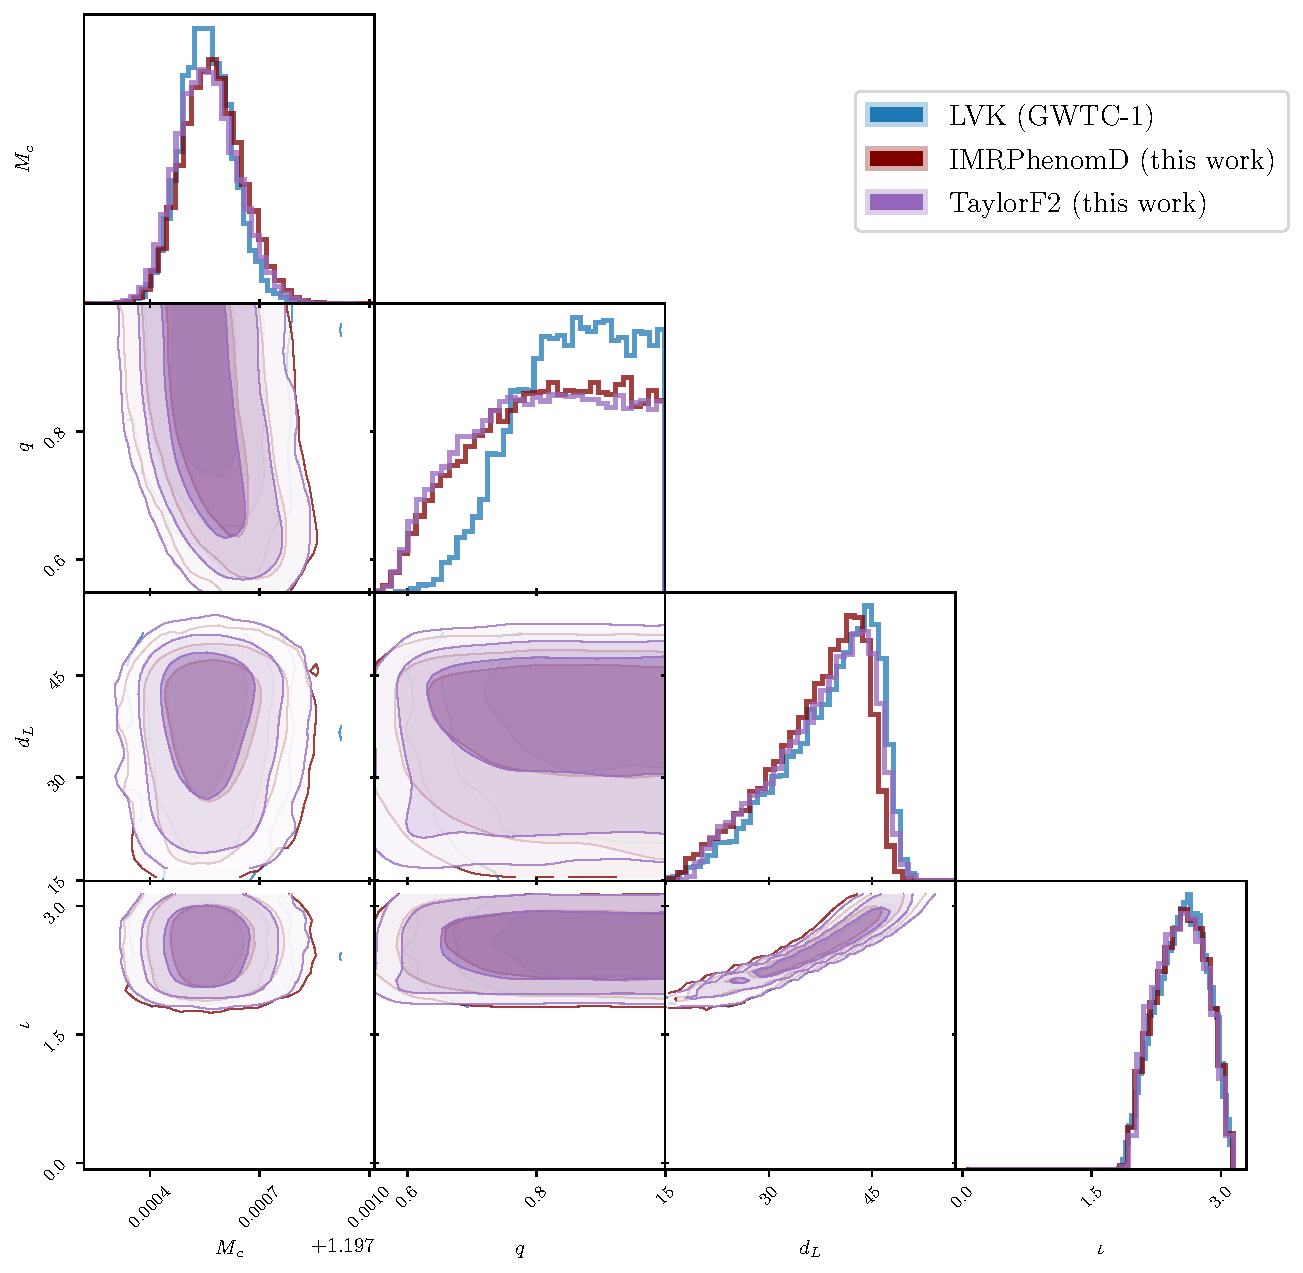
\includegraphics[width=0.92\textwidth]{corner_combined_waveforms.pdf}
  \caption{GW170817 source-parameter posteriors under \IMR and \TF in the heterodyned baseline configuration, overlaid on GWTC-1 reference samples. Produced by \texttt{Plots/plot\_corner\_combined\_waveforms.py}.}
  \label{fig:combined}
\end{figure*}

% ======================================================================
\section{Results}
\label{sec:results}

\subsection{Baseline Hubble-constant posterior}
\label{sec:baseline}

Under the baseline volumetric distance prior, the \IMR analysis yields a broad, asymmetric \hzero posterior. The maximum-posterior value is
\begin{equation}
\hzero^{\rm MAP} = 71.5\kmsmpc,
\end{equation}
with weighted 68 per cent quantile interval
\begin{equation}
\hzero \in [68.2,103.5]\kmsmpc \quad\text{(68\% q.i.)},
\end{equation}
and weighted median $79.1\kmsmpc$ [Source: \texttt{Results/gwtc1\_phasemarg/summary\_stats.csv}]. A kernel-density estimate of the 68 per cent highest-posterior-density interval gives $[62.7,91.1]\kmsmpc$; we report both the weighted-quantile and KDE-HPD forms because the posterior is strongly asymmetric and the two statistics emphasise different parts of the distribution. Figure~\ref{fig:h0baseline} shows the baseline posterior with Planck and SH0ES reference bands for context (TODO: verify the exact Planck and SH0ES values/intervals used in the figure against the current literature before submission).

\begin{figure}
  \centering
  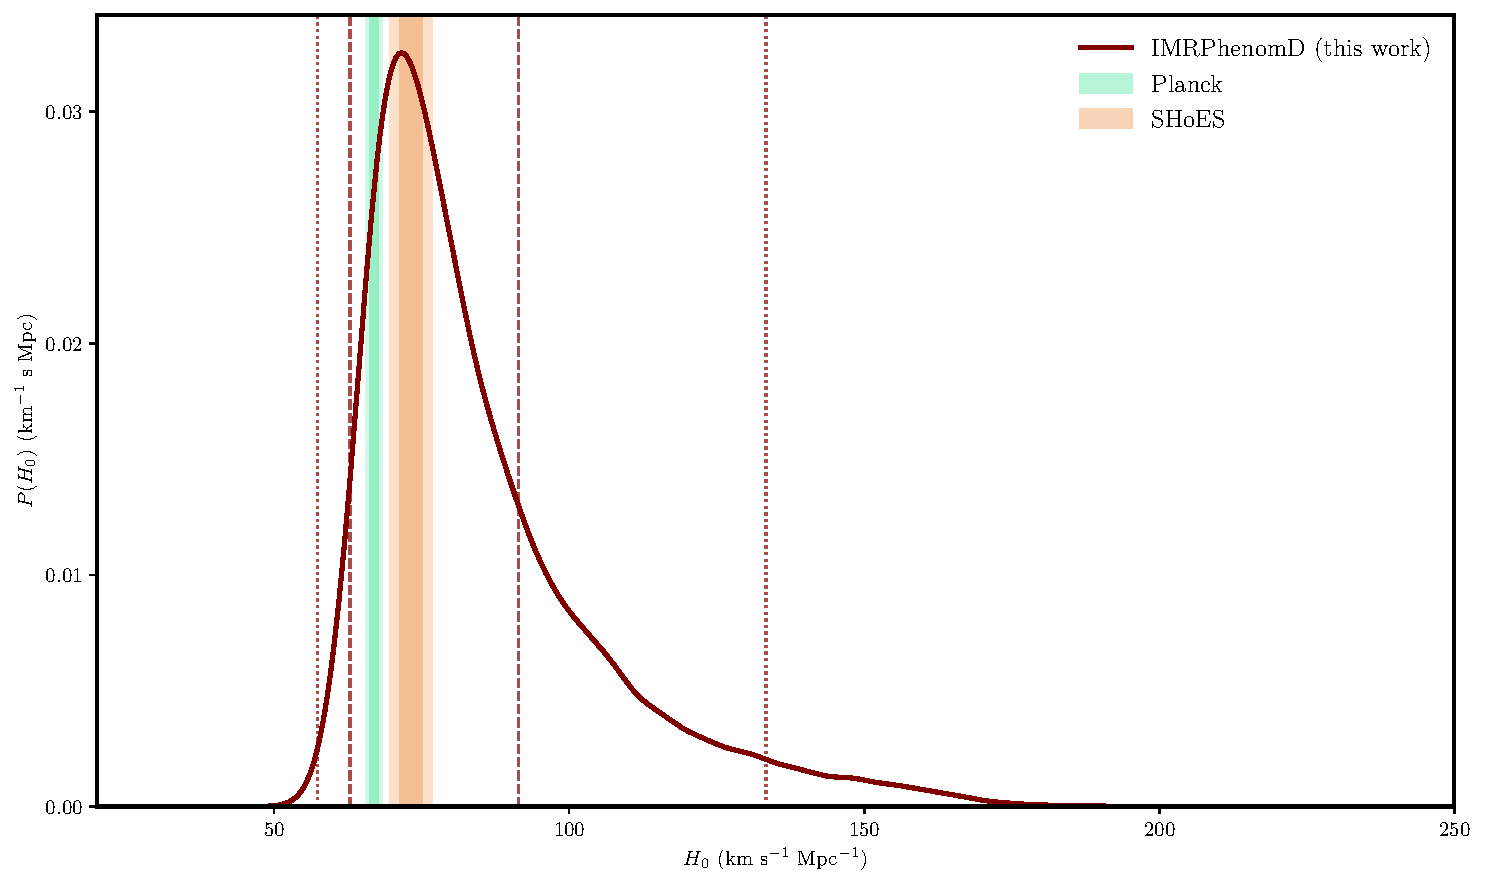
\includegraphics[width=\columnwidth]{H0_baseline_IMRPhenomD.pdf}
  \caption{Baseline GW170817 \hzero posterior under the volumetric distance prior with \IMR and 5000 live points. Shaded bands mark reference CMB and distance-ladder values (see text). Produced by \texttt{Plots/plot\_H0\_baseline\_IMRPhenomD.py} from \texttt{Results/gwtc1\_phasemarg/PhaseMarg\_Heterodyned\_IMRPhenomD\_NRTidalv2\_local\_psd-gwtc1\_ref-gwtc1\_baseline.csv}.}
  \label{fig:h0baseline}
\end{figure}

This posterior reproduces the qualitative features of the original GW170817 bright-siren measurement \citep{Abbott2017H0}: the peak is in the neighbourhood of the distance-ladder value, the posterior is broad enough to remain consistent with CMB measurements, and the high-\hzero tail extends to the upper edge of the prior range. The present analysis does not sharpen the single-event \hzero constraint relative to the literature; the purpose of reporting this posterior is to establish the baseline against which the prior-sensitivity comparison in Section~\ref{sec:prior} is performed.

\subsection{Prior sensitivity and the reweighting test}
\label{sec:prior}

The central scientific result of this paper is a direct comparison between the flat-in-redshift \hzero posterior obtained by sampling and that obtained by reweighting the baseline posterior to the same target prior. Table~\ref{tab:h0priors} summarises the four \IMR \hzero posteriors.

\begin{table*}
  \centering
  \caption{Primary \IMR \hzero summaries for the baseline volumetric-distance prior, the directly sampled and reweighted flat-in-redshift priors, and the enlarged peculiar-velocity variant. Weighted MAP, weighted median, weighted 68 per cent quantile intervals, 68 per cent KDE highest-posterior-density intervals, and two tail probabilities are shown.}
  \label{tab:h0priors}
  \begin{tabular}{lcccccc}
    \toprule
    Run & MAP & Median & 68\% quantile & 68\% KDE HPD & $P(\hzero>120)$ & $P(\dL<30\,\rm Mpc)$ \\
    \midrule
    Baseline (volumetric) & 71.5 & 79.1 & $[68.2,103.5]$ & $[62.7,91.1]$ & 0.076 & 0.179 \\
    Flat-in-$z$, direct   & 75.4 & 93.6 & $[72.4,146.9]$ & $[61.9,117.5]$ & 0.281 & 0.428 \\
    Flat-in-$z$, reweighted & 74.2 & 88.9 & $[71.3,126.2]$ & $[63.4,107.6]$ & 0.195 & 0.357 \\
    $\sigmavp=250\kms$    & 72.4 & 78.6 & $[67.0,101.9]$ & $[61.3,91.3]$ & 0.067 & 0.163 \\
    \bottomrule
  \end{tabular}
  \\ \footnotesize[Source: \texttt{Results/gwtc1\_phasemarg/summary\_stats.csv}; \texttt{Results/gwtc1\_phasemarg/prior\_sensitivity.csv}; \texttt{paper\_knowledge\_base/a100\_run\_data.md}. All \hzero values are in $\kmsmpc$.]
\end{table*}

\begin{figure}
  \centering
  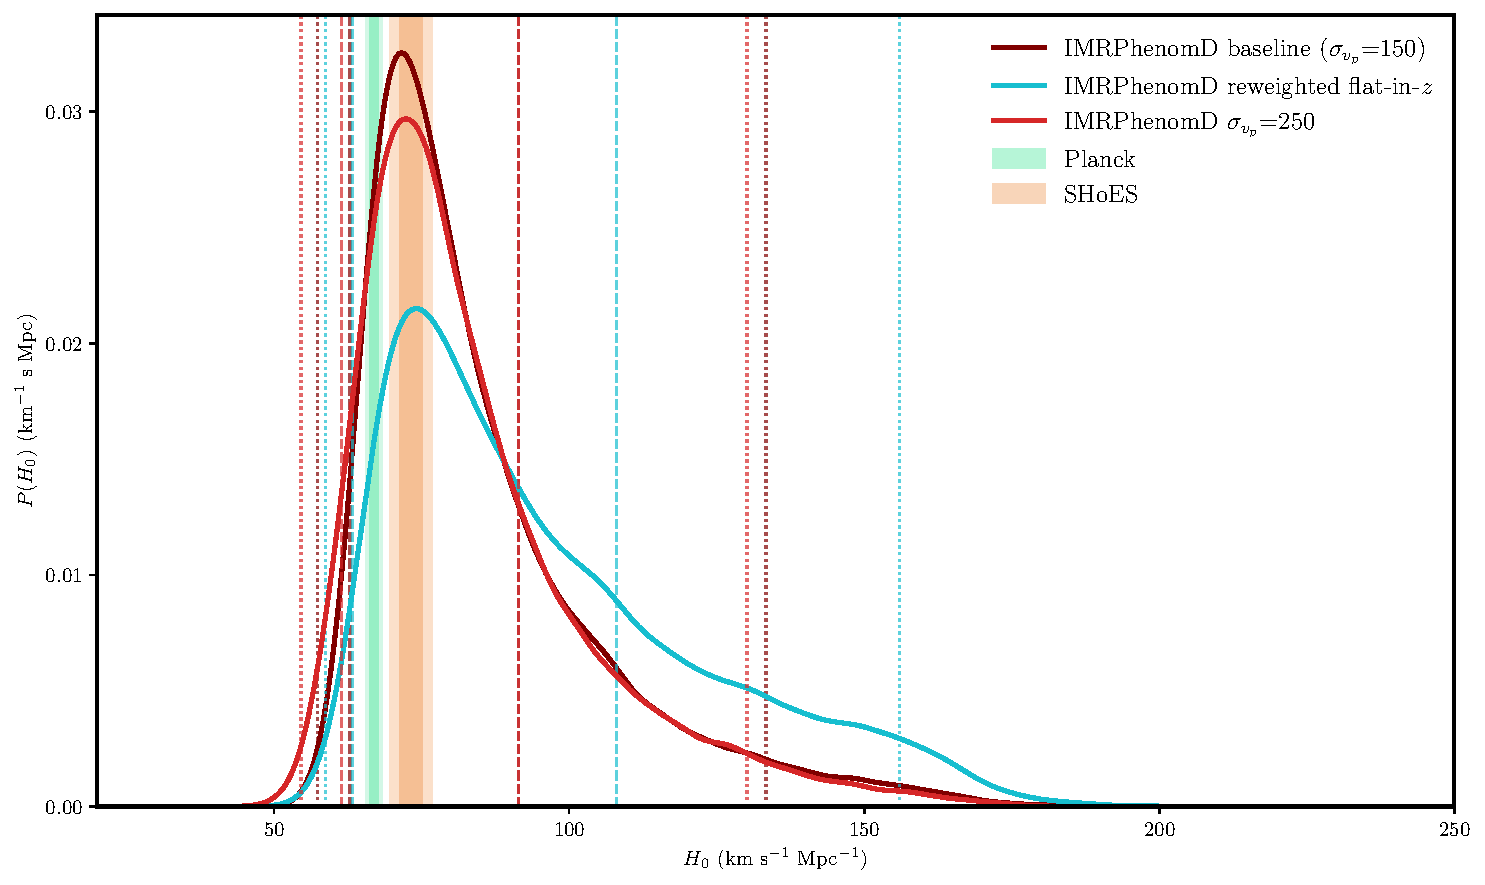
\includegraphics[width=\columnwidth]{H0_IMRPhenomD_reweighted.pdf}
  \caption{Prior-sensitivity comparison for \IMR. The directly sampled flat-in-redshift posterior (teal) places substantially more mass at high \hzero than the reweighted baseline posterior (dashed), and both shift to higher \hzero than the baseline volumetric-distance posterior (solid). The enlarged peculiar-velocity run (dotted) is effectively indistinguishable from the baseline in this projection. Produced by \texttt{Plots/plot\_H0\_IMRPhenomD\_reweighted.py}.}
  \label{fig:h0prior}
\end{figure}

The direct flat-in-redshift run shifts the weighted median from $79.1$ to $93.6\kmsmpc$ and broadens the 68 per cent quantile interval by about a factor of $2$ on the high side. The reweighted flat-in-redshift posterior moves in the same direction but by a smaller amount: its weighted median is $88.9\kmsmpc$ and its 68 per cent quantile interval reaches $126.2\kmsmpc$ rather than $146.9\kmsmpc$. The difference is sharpest in the high-\hzero tail: the probability
\begin{equation*}
P(\hzero>120\kmsmpc) \;=\; 0.076,\ 0.195,\ 0.281
\end{equation*}
for the baseline, reweighted and directly sampled posteriors respectively; $P(\hzero>150\kmsmpc)$ rises from $0.016$ in the baseline to $0.056$ in the reweighted posterior and $0.147$ in the direct posterior [Source: \texttt{Results/gwtc1\_phasemarg/prior\_sensitivity.csv}]. The earth-mover (Wasserstein-1) distance of each posterior from the baseline is $11.2\kmsmpc$ for reweighting and $20.8\kmsmpc$ for direct sampling. In the sense of cumulative distribution, the reweighted posterior is therefore only about half of the way to the direct flat-in-redshift posterior. Figure~\ref{fig:h0prior} visualises this hierarchy.

The mechanism is directly visible in the luminosity-distance marginal, shown in Figure~\ref{fig:dlreweight}. A flat-in-redshift prior up-weights small \dL relative to the baseline volumetric prior; small \dL in turn maps to large \hzero for the fixed host recessional velocity. In the direct run, the sampler explores the low-\dL region with live points drawn from the flat-in-redshift prior, and the posterior accumulates weight there. The probability $P(\dL<30\,\rm Mpc)$ rises from $0.179$ in the baseline to $0.428$ in the direct flat-in-redshift posterior. In the reweighted run, the baseline samples are re-scored by the prior ratio, but there are few baseline samples at low \dL because the baseline volumetric prior had placed little probability there in the first place. The reweighted estimator consequently under-represents the low-\dL region ($P(\dL<30\,\rm Mpc)=0.357$) and, as a consequence, under-represents the high-\hzero region. Corner comparisons in the \dL--$\iota$ plane confirm that the direct and reweighted posteriors differ mainly in the low-\dL, small-$\iota$ corner; the waveform-parameter marginals are almost identical [Source: \texttt{Results/gwtc1\_phasemarg/plots/corner\_reweighted\_vs\_sampled\_flatZ\_IMRPhenomD.pdf}, produced by \texttt{Plots/plot\_corner\_reweighted\_vs\_sampled\_flatZ.py}].

\begin{figure}
  \centering
  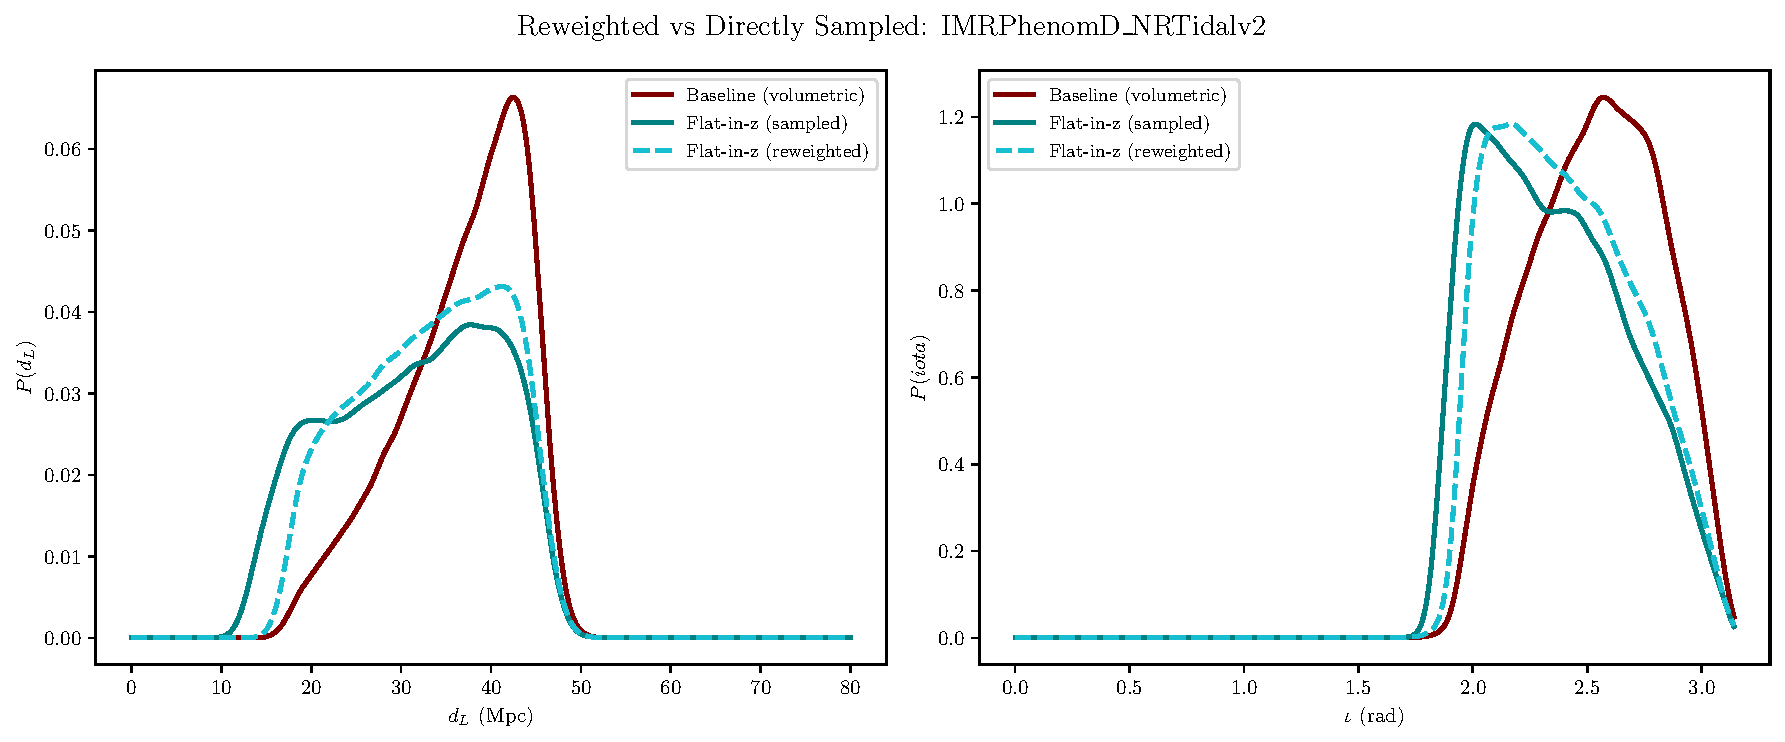
\includegraphics[width=\columnwidth]{dL_reweight_comparison_IMRPhenomD_NRTidalv2.pdf}
  \caption{Luminosity-distance posterior for \IMR under the baseline volumetric prior (solid), the directly sampled flat-in-redshift prior (teal), and the reweighted baseline posterior (dashed). The direct run places substantially more mass at $\dL\lesssim30\,\rm Mpc$, which maps to higher \hzero through the host-galaxy velocity relation. Produced by \texttt{Plots/compute\_prior\_sensitivity.py} with \texttt{WAVEFORM=IMRPhenomD\_NRTidalv2}.}
  \label{fig:dlreweight}
\end{figure}

The enlarged peculiar-velocity variant ($\sigmavp=250\kms$) shifts the \hzero posterior only slightly: the median falls marginally to $78.6\kmsmpc$ and the high-\hzero tail thins, giving $P(\hzero>120)=0.067$. The Wasserstein distance from the baseline is $1.24\kmsmpc$, an order of magnitude smaller than either flat-in-redshift comparison. For GW170817 with NGC~4993 identified, the dominant prior-induced uncertainty in \hzero is therefore the distance prior, not the peculiar-velocity uncertainty.

We caution against over-interpreting these shifts as physical results for \hzero. None of them changes the qualitative statement that GW170817 alone is consistent with both early- and late-Universe measurements of the expansion rate. The scientific content is that the magnitude of the shift under a change of distance prior is a property of the inference, not of the cosmology, and that the magnitude one would report using reweighting alone is materially different from the magnitude recovered by direct sampling.

\subsection{Waveform cross-check}
\label{sec:waveform}

Repeating the same four analyses with \TF gives qualitatively identical prior dependence. The \TF baseline weighted median is $77.7\kmsmpc$ with 68 per cent quantile interval $[66.8,101.9]\kmsmpc$, and the direct flat-in-redshift run has weighted median $87.8\kmsmpc$ with interval $[70.0,127.1]\kmsmpc$ [Source: \texttt{Results/gwtc1\_phasemarg/summary\_stats.csv}]. Jensen--Shannon divergences between IMR and TF2 are $0.005$ and $0.014\,\rm nats$ for the baseline and flat-in-redshift \hzero posteriors, respectively [Source: \texttt{Results/gwtc1\_phasemarg/waveform\_systematics.csv}]. The waveform-induced \hzero shift therefore remains smaller than the prior-induced shift, even though \TF is a post-Newtonian inspiral-only approximant without tidal terms in our implementation and the \IMR family incorporates NR-calibrated tides. The reweighting-versus-direct-sampling discrepancy persists in TF2: the direct flat-in-redshift median is $87.8\kmsmpc$ against $87.4\kmsmpc$ for reweighting, but the 68 per cent quantile reaches $127.1\kmsmpc$ directly against $120.5\kmsmpc$ reweighted. This mirrors the \IMR behaviour and indicates that the effect is governed by the distance-prior geometry rather than by the waveform.

\subsection{Evidence}
\label{sec:evidence}

The nested-sampling evidence for each run is summarised in Table~\ref{tab:evidence}. Within \IMR, the baseline and flat-in-redshift evidences differ by $0.18$ in $\ln Z$ with run-to-run uncertainty of order $0.1$, and the $\sigmavp=250\kms$ run differs by $-0.71$ from the baseline. On the Jeffreys scale these are not decisive, and repeat-run evidence values in the repository fluctuate at the same level [Source: \texttt{paper\_knowledge\_base/a100\_run\_data.md}, Run Sets 1 and 2]. The \TF run evidences are all higher than the \IMR values by $\approx0.3$--$0.7$ in $\ln Z$; this is expected because of the different waveform phase evolution and does not constitute evidence against the tidal waveform for this single event. We report $\ln Z$ values for completeness and caution that the current data do not prefer one prior configuration or waveform at a statistically meaningful level.

\begin{table}
  \centering
  \caption{Nested-sampling evidences for the six heterodyned GW170817 runs. Quoted uncertainties are the BlackJAX-NS statistical estimates on a single run; intrinsic run-to-run variation from \texttt{paper\_knowledge\_base/a100\_run\_data.md} is of the same order.}
  \label{tab:evidence}
  \begin{tabular}{lc}
    \toprule
    Run & $\ln Z$ \\
    \midrule
    \IMR, baseline              & $486.67\pm0.09$ \\
    \IMR, flat-in-$z$, direct   & $486.49\pm0.10$ \\
    \IMR, $\sigmavp=250\kms$    & $485.96\pm0.08$ \\
    \TF, baseline               & $486.90\pm0.10$ \\
    \TF, flat-in-$z$, direct    & $487.18\pm0.09$ \\
    \TF, $\sigmavp=250\kms$     & $487.28\pm0.08$ \\
    \bottomrule
  \end{tabular}
  \\ \footnotesize[Source: \texttt{Results/gwtc1\_phasemarg/evidence\_table.csv}.]
\end{table}

% ======================================================================
\section{Performance}
\label{sec:performance}

The science-enabling claim of this paper is that fast nested sampling makes the prior-sensitivity test of Section~\ref{sec:prior} practical. This section quantifies the runtime on a single A100 GPU (Google Cloud a2-highgpu-1g instance [Source: \texttt{paper\_knowledge\_base/hardware\_platforms.md}]), without attempting a like-for-like CPU benchmark.

\subsection{Wall-clock runtime}

The primary heterodyned GW170817 \hzero analysis with \IMR and 5000 live points completes in 14\,min 45\,s of wall-clock time, of which 12\,min 52\,s is the sampling stage and the remaining $\sim2\,\rm min$ is data loading, heterodyne setup, sampler initialisation and JIT compilation [Source: \texttt{paper\_knowledge\_base/a100\_run\_data.md}]. The corresponding \TF baseline completes in 3\,min 55\,s total ($2\,\rm min\,41\,s$ sampling). The full six-run prior-sensitivity suite---baseline, direct flat-in-redshift, and $\sigmavp=250\kms$ for both waveforms---completes in $\approx57\,\rm min$ end to end. The GW150914 validation run in Section~\ref{sec:validation} takes 4\,min 8\,s total. These numbers are for the same hardware that produced all posterior CSV files used in the preceding sections, so the runtime quoted for each posterior is the runtime of the run that produced it.

The heterodyned likelihood is the enabling approximation. A head-to-head comparison on the same A100 hardware shows that an unheterodyned \IMR GW170817 run with 1500 live points and host-localised priors requires 5\,h 34\,min of wall-clock time; the heterodyned run at $3.3\times$ more live points completes in 14\,min 45\,s. At matched configurations, sampling-only speedups in the range $\sim$21--26$\times$ for \IMR and $\sim$28--53$\times$ for \TF are recorded in the repository [Source: \texttt{paper\_knowledge\_base/a100\_run\_data.md}]. These numbers establish that the relative-binning approximation is responsible for the order-of-magnitude reduction in runtime, and that the GPU contribution, while important for keeping the sampler saturated, is layered on top of the algorithmic improvement.

\subsection{Scaling with live points}

\begin{figure}
  \centering
  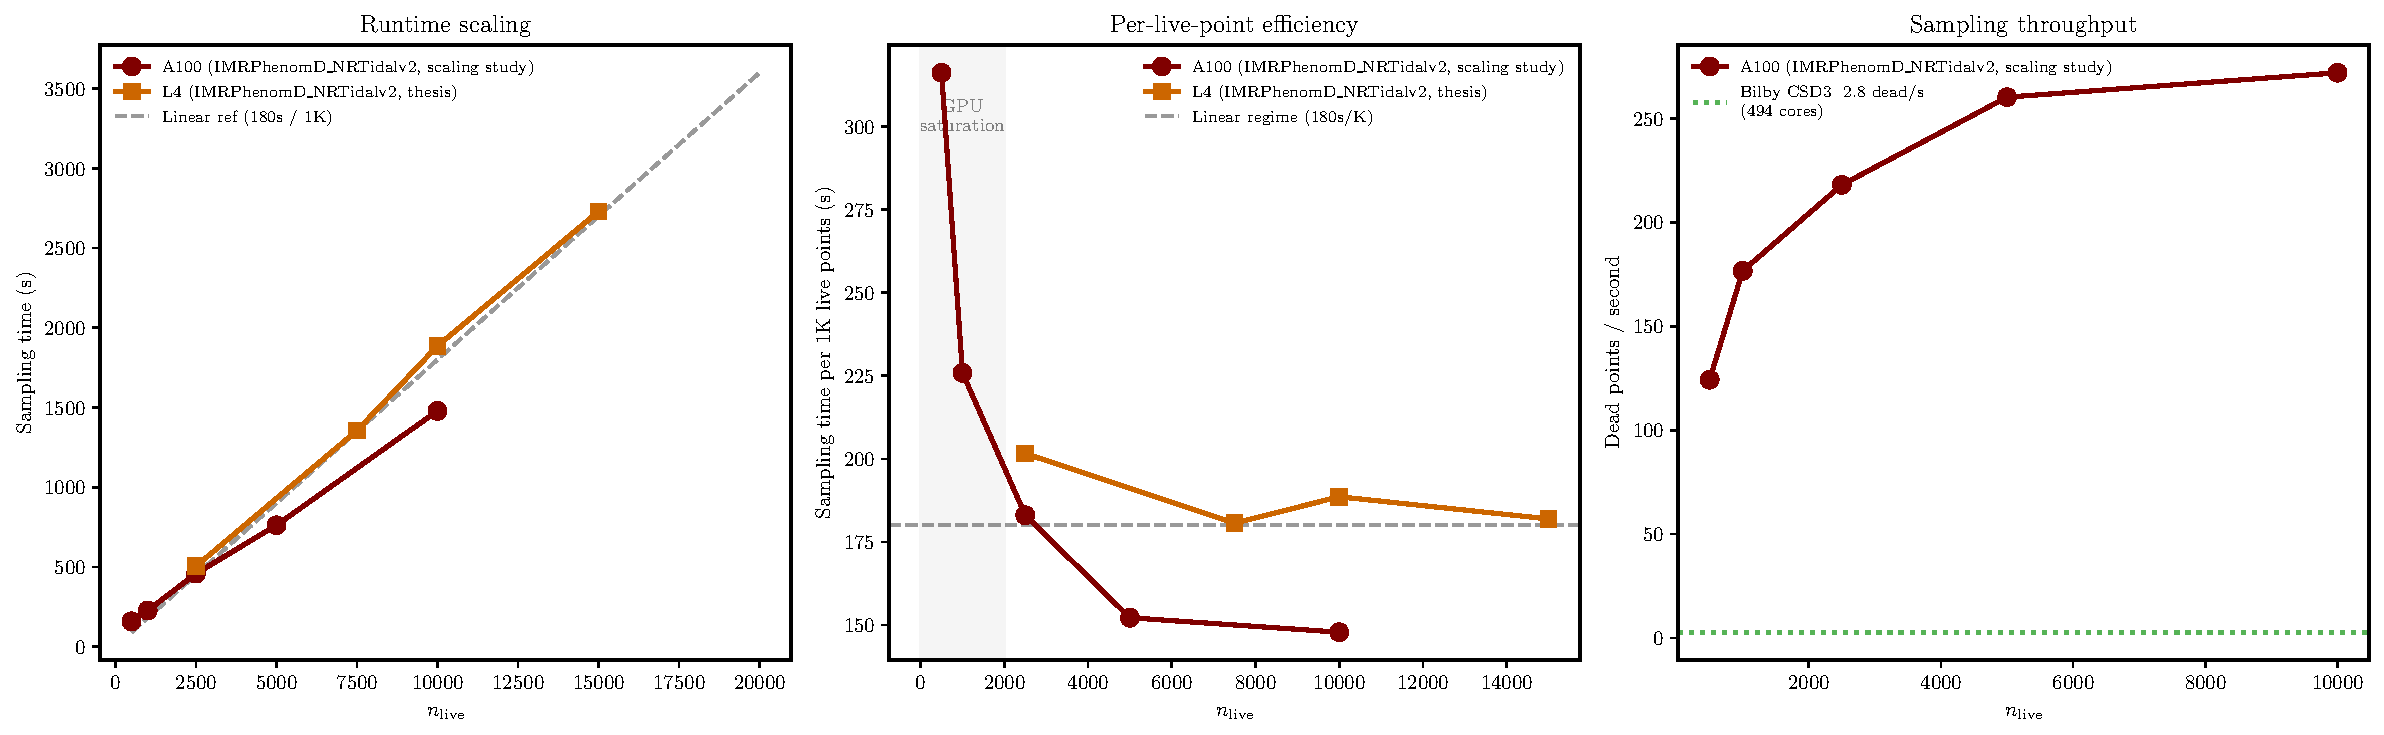
\includegraphics[width=\columnwidth]{scaling_study.pdf}
  \caption{Wall-clock runtime of the heterodyned \IMR GW170817 analysis as a function of nested-sampling live-point count, on a single A100 GPU. Total runtime is shown; data loading, heterodyne setup, initialisation and JIT compilation contribute an approximately live-point-independent overhead of $\sim80\,\rm s$. Produced by \texttt{Plots/plot\_scaling\_study.py} from \texttt{Results/scaling\_study/scaling\_summary.csv}.}
  \label{fig:scaling}
\end{figure}

Table~\ref{tab:scaling} and Figure~\ref{fig:scaling} show the live-point scaling of the heterodyned \IMR analysis. The 5000-live-point configuration used for the science runs sits in the middle of the accessible range. At 100\,000 live points the analysis still completes within four hours on a single A100, and the statistical uncertainty on the evidence falls to $\sigma_{\ln Z}=0.02$.

\begin{table}
  \centering
  \caption{Live-point scaling of the heterodyned \IMR GW170817 analysis on a single A100 GPU. Dead points are the total number accumulated at sampler termination.}
  \label{tab:scaling}
  \begin{tabular}{rrrrrr}
    \toprule
    $n_{\rm live}$ & Dead pts & $\ln Z$ & $\sigma_{\ln Z}$ & Sampling (s) & Total (s) \\
    \midrule
    500     & $19\,650$   & 486.73 & 0.30 & 158    & 235     \\
    1000    & $39\,900$   & 486.04 & 0.21 & 226    & 304     \\
    2500    & $99\,750$   & 486.32 & 0.13 & 458    & 550     \\
    5000    & $198\,000$  & 486.66 & 0.10 & 761    & 872     \\
    10\,000 & $402\,000$  & 485.92 & 0.07 & 1478   & 1659    \\
    20\,000$^{\dagger}$ & $690\,000$  & 485.95 & 0.05 & 1695  & 2035    \\
    50\,000 & $1\,725\,000$ & 486.22 & 0.03 & 4812 & 6280    \\
    100\,000 & $3\,450\,000$ & 486.29 & 0.02 & 9150 & 14\,393 \\
    \bottomrule
  \end{tabular}
  \\ \footnotesize[Source: \texttt{Results/scaling\_study/scaling\_summary.csv}.] $^{\dagger}$The $n_{\rm live}=20\,000$ entry accumulates fewer dead points than a strict linear extrapolation from the surrounding rows would suggest; the scaling plot is drawn without relying on this point for a linear-scaling claim and the discrepancy is noted as an open item (see \S\ref{sec:discussion}).
\end{table}

Runtime scales close to linearly with live-point count once the sampler is saturated ($n_{\rm live}\gtrsim2500$), consistent with the sampler-bound regime discussed in \citet{Prathaban2025GPUSpeed}. Below that, the fixed overhead per iteration dominates. The 5000-live-point configuration is therefore comfortably within the linear-scaling regime, and the science runs are not under-sampled: the baseline produces $\sim2\times10^{5}$ dead points and an effective sample size of $\sim3.7\times10^{4}$ [Source: \texttt{Results/gwtc1\_phasemarg/evidence\_table.csv}].

\subsection{Scope of the performance claim}

We deliberately do not compare runtime against a single-core CPU baseline, which would give a misleadingly large speedup factor, nor against a production \pbilby run that we have not executed under matched settings. A like-for-like GW170817 \pbilby benchmark using \IMR with identical priors, live-point count, and waveform configuration is the appropriate CPU comparison and is left for future work (TODO: insert the matched \pbilby benchmark once executed on CSD3). The claim we do make is narrower and reproducible: on a single A100 GPU, the full 5000-live-point GW170817 \hzero analysis completes in under a quarter of an hour, and a six-run prior-sensitivity suite fits inside one hour. This runtime budget is what makes the direct comparison with reweighting in Section~\ref{sec:prior} scientifically routine rather than exceptional.

% ======================================================================
\section{Discussion}
\label{sec:discussion}

\subsection{Implications for bright-siren cosmology}

The main methodological message of our analysis is that posterior reweighting, although statistically consistent in the limit of infinite baseline samples, can substantially understate the prior sensitivity of bright-siren \hzero measurements in practice. For GW170817, switching from a volumetric-distance prior to a flat-in-redshift prior changes $P(\hzero>120\kmsmpc)$ by a factor of about $3.7$ under direct sampling, and by about $2.6$ under reweighting. The reweighted estimator therefore misses nearly half of the prior-induced change in the tail of the posterior, because the baseline volumetric prior places little probability at the low-\dL values that the flat-in-redshift prior up-weights. This is a problem of effective sample coverage rather than of statistical methodology. It is an expected outcome once the mechanism is articulated, but it is not the behaviour that would be inferred from a reweighting-only analysis.

For a single event, this under-estimation does not change the cosmological interpretation: the GW170817 posterior is broad enough that both early-Universe and late-Universe \hzero values lie within its 68 per cent credible interval under any of the prior choices considered here. However, the scale of the prior-sensitivity effect matters for forecasts and combined analyses. When bright-siren posteriors are combined over multiple events, or when tail probabilities are compared against external priors from cosmological surveys, the prior-dependence of each single-event posterior propagates through. An analysis that quantifies that dependence only through reweighting risks a systematic bias in the direction of underestimating the prior contribution.

\subsection{Where reweighting is sufficient}

Reweighting is adequate when the target and baseline priors have similar support in the regions that carry most of the posterior mass. The $\sigmavp=250\kms$ variant in our analysis is a case of this kind: the change in \sigmavp modifies the host-velocity likelihood smoothly over the scale of the velocity posterior, the baseline samples cover the affected region well, and the reweighted and directly sampled \sigmavp posteriors agree to well within the statistical width (Wasserstein distance $1.2\kmsmpc$). The flat-in-redshift case fails the same coverage test, because the baseline volumetric prior and the target flat-in-redshift prior differ most at the edges of the \dL range. Diagnostics such as an effective-sample-size ratio under the reweighted weights, or a direct overlay of the \dL marginals, can flag such cases before the reweighted \hzero posterior is reported.

\subsection{Implications for future bright sirens}

The practical consequence is that direct prior sampling should be used for bright-siren \hzero analyses whenever the target prior differs non-trivially in support from the baseline, rather than being used only as a cross-check. The runtime budget on a single A100 GPU now permits such reruns routinely, and the scaling study in Section~\ref{sec:performance} indicates that live-point counts up to $10^{5}$ are accessible on the same hardware, which means that prior-sensitivity studies can in principle be combined with population-level analyses without a substantial increase in end-to-end wall-clock time. This is directly relevant to the third-generation detector era, where the detection rate of compact-binary mergers will make repeated, controlled posterior reanalyses the norm rather than the exception \citep{HuVeitch2025}.

\subsection{Limitations and open items}

Several limitations should be addressed before the present analysis is treated as a definitive prior-sensitivity study.

First, the primary waveform in our analysis, \IMR, is aligned-spin and does not include precession; the original GW170817 bright-siren analysis used the precessing IMRPhenomPv2\_NRTidal family. Precession is expected to be subdominant for GW170817 given NGC~4993's sky localisation and the modest spin constraints allowed by the source priors, but we do not claim a precessing analysis here, and any quantitative statement about precession effects on the \hzero prior sensitivity would require an additional sampler with a precessing waveform in \jax.

Second, the host-galaxy association with NGC~4993, its recessional velocity, and the peculiar-velocity estimate are taken directly from the bright-siren setup of \citet{Abbott2017H0}. We have varied \sigmavp but have not varied $\langle v_{p}\rangle$; systematic work on host-galaxy peculiar velocities is outside the scope of this paper.

Third, we do not present a matched \pbilby benchmark. The performance claim is therefore explicitly restricted to single-A100 wall-clock runtime and scaling on the current pipeline (\S\ref{sec:performance}), and any CPU-vs-GPU comparison is deferred.

Fourth, the $n_{\rm live}=20\,000$ scaling-study entry (Table~\ref{tab:scaling}) accumulates fewer dead points than a linear interpolation from neighbouring runs would predict. This is an open item; we have not used this row for any scaling claim and the discrepancy should be investigated before the scaling table is treated as definitive.

Finally, several reference-sample cross-comparisons, notably against GWTC-1 and GWTC-2.1 public posteriors, are shown in corner form only. Direct \hzero comparisons against updated LVK reanalyses would sharpen the context for Section~\ref{sec:prior}, but are not a prerequisite for the methodological conclusion.

% ======================================================================
\section{Conclusions}
\label{sec:conclusions}

We have used a GPU-native nested-sampling pipeline to carry out a direct prior-sensitivity analysis of the Hubble-constant measurement from GW170817. The baseline \IMR analysis yields a broad \hzero posterior with maximum-posterior value $71.5\kmsmpc$ and 68 per cent weighted quantile interval $[68.2,103.5]\kmsmpc$, consistent with the original bright-siren result. Switching from the baseline volumetric-distance prior to a flat-in-redshift prior by direct sampling produces a substantially broader posterior with weighted median $93.6\kmsmpc$ and a high-\hzero tail probability $P(\hzero>120\kmsmpc)=0.281$. Reweighting the baseline posterior to the same target prior gives $P(\hzero>120\kmsmpc)=0.195$, only partially capturing the shift, because the baseline samples under-populate the low-\dL region that the target prior up-weights. The waveform cross-check with \TF and a modified peculiar-velocity uncertainty both produce smaller shifts than the distance-prior change. The analysis runs in 14\,min 45\,s on a single A100 GPU, and the full six-run prior-sensitivity suite in 57\,min. The scientific value of fast nested sampling for bright-siren cosmology is that direct prior reruns replace post-hoc reweighting as the default robustness tool, without a substantial change in the computational budget.

% ======================================================================
\section*{Acknowledgements}

TODO: add supervisor, research-group, compute-resource (Google Cloud A100), and funding acknowledgements; acknowledge GWOSC (TODO: insert appropriate GWOSC data-release citation) and the LIGO--Virgo--KAGRA Collaboration for the public strain data and reference posteriors used here.

% ======================================================================
\section*{Data Availability}

This paper uses publicly available GW170817 and GW150914 strain data and GWTC-1 and GWTC-2.1 reference posteriors from the Gravitational Wave Open Science Center (GWOSC). All derived posterior-sample CSV files, summary tables, scaling logs, and plotting scripts used in this paper are distributed with the project repository at \url{TODO: insert permanent repository URL/DOI}, and are listed by provenance in \texttt{paper\_knowledge\_base/result\_link\_index.md}. Large CSVs and HDF5 reference files are tracked with Git LFS; detailed regeneration instructions are in \texttt{Plots/run\_all\_plots.sh}. TODO: confirm GWOSC release identifiers for the GW170817 and GW150914 strain segments before submission.

% ======================================================================
\bibliographystyle{mnras}
\bibliography{references}

\label{lastpage}
\end{document}
